\section{Results and Discussion}
\label{sec:results}
\subsection{Main comparison}
\label{sec:main_results}
Tables~\ref{tab:main} and~\ref{tab:main_auroc} compare \ours{} with all baselines at $k=25$ (other $k$ and all metrics:
Supplementary Section~\sref{app:full}).

\begin{table}[t]\centering
\caption{\textbf{Main comparison, macro-F1} at $k=25$ labelled words per class (learned methods: ensemble of five
seeds; threshold baselines: mean over the five supports). FUNSD and CORD were used for development; SROIE, IAM and
IIIT5K are held out. $^\dagger$Threshold tuned on the test set (upper bound); $^\ddagger$the best baseline chosen
separately for every dataset in hindsight (both excluded from the colour marks).}
\label{tab:main}
\scriptsize\setlength{\tabcolsep}{6pt}
\begin{tabular}{lcccccc}\toprule
Method & FUNSD & CORD & SROIE & IAM & IIIT5K & Avg.\\\midrule
\tabinput{tables/main_macro_f1_k25.tex}
\bottomrule\end{tabular}
\end{table}

\begin{table}[t]\centering
\caption{\textbf{Main comparison, AUROC} at $k=25$ (same protocol as Table~\ref{tab:main}).}
\label{tab:main_auroc}
\scriptsize\setlength{\tabcolsep}{6pt}
\begin{tabular}{lcccccc}\toprule
Method & FUNSD & CORD & SROIE & IAM & IIIT5K & Avg.\\\midrule
\tabinput{tables/main_auroc_k25.tex}
\bottomrule\end{tabular}
\end{table}

\textbf{General-purpose verifiers are far from sufficient.} Engine confidence, its learned refinement, engine voting,
Florence-2 re-recognition and the 7B VLM judge all trail \ours{} by large margins on every dataset. Despite 8.3B
parameters the VLM judge reaches only \VLMFUNSD{} macro-F1 on FUNSD and \VLMIAM{} on IAM, and an oracle threshold barely
helps: its errors are errors of \emph{ranking}, not of calibration. Character-exact judgements (\texttt{O} vs.\
\texttt{0}, a missing comma, a case flip) are what instruction-tuned VLMs gloss over.

\textbf{Re-recognition with a strong recogniser is the baseline to beat.} Accepting a claim iff PARSeq reads the same
string is by far the strongest baseline, and its graded variant more so. \ours{} improves on it where PARSeq is
fallible: on IAM handwriting by \GAINIAMFone{} macro-F1 and \GAINIAMauc{} AUROC, and on CORD receipts (macro-F1
\LOCUSCORDfone{} vs.\ \PQCORDfone{}; AUROC gain significant, Table~\ref{tab:significance}). On FUNSD the two are
statistically tied, and on IIIT5K, the scene-text benchmark on which PARSeq was designed and reads almost every word
correctly, PARSeq agreement remains better (\PQIIITfone{} vs.\ \LOCUSIIITfone{}). \SROIESENTENCE

\textbf{Learned baselines on our evidence and the label-free model.} Logistic regression, gradient boosting and
DeepSets on the \emph{same} counterfactual evidence are competitive with \ours{} (middle blocks): most of the gain over
general-purpose baselines comes from the counterfactual, render-normalised \emph{evidence} itself, and
Section~\ref{sec:mp} shows that message passing adds little on top of it. Pretrained only on engine agreement and
synthetic corruptions, zero-shot \ours{} already exceeds engine confidence, learned confidence, Florence-2 and the VLM
judge in AUROC on every dataset, and engine voting on four of five (all except SROIE, where both voting engines include a
SROIE-trained recogniser).

\begin{figure}[t]\centering
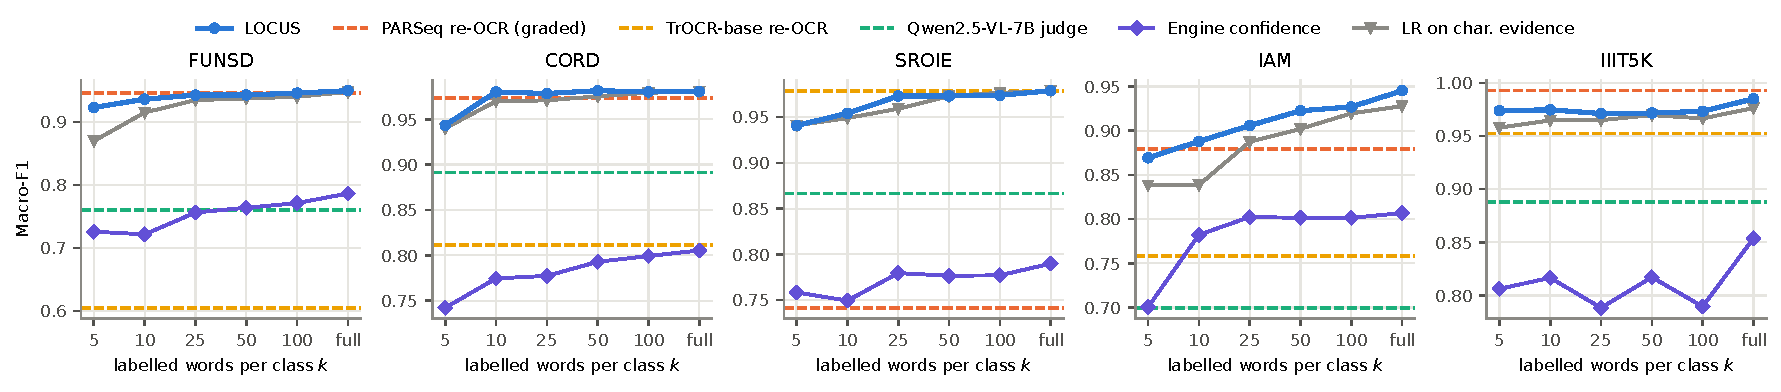
\includegraphics[width=0.8\linewidth]{figs/learning_curves_macro_f1.pdf}
\caption{\textbf{Label efficiency.} Macro-F1 versus labelled words per class (ensembles of five seeds; dashed:
label-free baselines). AUROC curves: Supplementary Figure~\sref{fig:lc_auroc}.}
\label{fig:lc}
\end{figure}

\subsection{Label efficiency and render normalisation}
Figure~\ref{fig:lc} shows that \ours{} is close to its fully supervised accuracy with $k=10$--$25$ labelled words per
class on the document datasets, and keeps improving with more labels on IAM; seed variance shrinks rapidly with $k$
(Supplementary Section~\sref{app:full}). Supplementary Figure~\sref{fig:rho} isolates Equation~\eqref{eq:rho} on a single score: the raw TrOCR
likelihood of the claim is a poor detector wherever the recogniser's string prior is mismatched with the domain, and
subtracting the likelihood of the claim's own rendering repairs it. In the full model, where a second verifier and
agreement features overlap, removing render normalisation costs little (Table~\ref{tab:ablation}); with TrOCR as the
only verifier it helps where TrOCR's prior is mismatched (SROIE .956 vs.\ .902, CORD .973 vs.\ .967, IIIT5K .957 vs.\
.951), is neutral on FUNSD and slightly harmful on IAM, and with PARSeq alone it makes no difference
(Supplementary Table~\sref{tab:single}): render normalisation corrects a \emph{biased} recogniser and is neutral for an unbiased one.



\subsection{Ablations}
\label{sec:ablation}
\begin{table}[t]\centering
\caption{\textbf{Ablations} at $k=25$, macro-F1 (ensemble of five seeds). $\Delta$: mean change w.r.t.\ the full model
over the datasets where the variant was run (AUROC: Supplementary Table~\sref{tab:ablation_auroc}).}
\label{tab:ablation}
\scriptsize\setlength{\tabcolsep}{4.5pt}
\begin{tabular}{lcccccc}\toprule
Variant & FUNSD & CORD & SROIE & IAM & IIIT5K & $\Delta$\\\midrule
\tabinput{tables/ablation_macro_f1.tex}
\bottomrule\end{tabular}\end{table}



Table~\ref{tab:ablation} reports every component. The clearest effects are label-free pretraining and operating on the
edit graph at all (versus the same character evidence without rival hypotheses). Several conceptually central components
are individually \emph{redundant} in the full model: removing message passing, the local-optimality term, the repair
loss or render normalisation changes macro-F1 by less than a point on most datasets, because the two verifiers and the
agreement features carry overlapping information; GCN and GraphSAGE backbones perform like GATv2 and GIN is slightly
worse ($-0.009$). The value of \ours{} lies in \emph{what} is compared (the claim against its counterfactual rivals,
under prior-cancelled evidence) more than in the network that compares them.

\subsection{Transfer across engines and datasets}
\begin{table}[t]\centering
\caption{\textbf{Transfer.} Left: engine transfer (train on one engine's claims, test on the other's; in-engine:
trained and tested on the target engine). Right: dataset transfer, macro-F1 (rows: training dataset, fully
supervised; shaded: in-domain).}
\label{tab:xengine}
\footnotesize\setlength{\tabcolsep}{2.6pt}
\begin{minipage}[t]{0.56\linewidth}\centering
\resizebox{\linewidth}{!}{\begin{tabular}{llcccccc}\toprule
& & \multicolumn{3}{c}{$k=25$} & \multicolumn{3}{c}{full}\\
Dataset & Train$\rightarrow$Test & F1 in & F1 tr. & AUROC tr. & F1 in & F1 tr. & AUROC tr.\\\midrule
\tabinput{tables/xengine.tex}
\bottomrule\end{tabular}}
\end{minipage}\hfill
\begin{minipage}[t]{0.42\linewidth}\centering
\resizebox{\linewidth}{!}{\begin{tabular}{lccccc}\toprule
Train$\backslash$Test & FUNSD & CORD & SROIE & IAM & IIIT5K\\\midrule
\tabinput{tables/xdataset_macro_f1.tex}
\bottomrule\end{tabular}}
\end{minipage}
\end{table}

A verifier that must be retrained for every engine is of limited use. Trained on Tesseract claims and tested on
TrOCR-small claims (and vice versa), the fully supervised \emph{ranking} transfers with an AUROC loss of at most 0.006 on
FUNSD, CORD and IIIT5K (at most 0.023 at $k=25$), but SROIE loses 0.02--0.07, and the 0.5 decision threshold transfers
poorly everywhere because the two engines' error rates and types differ; a new engine therefore needs at least
threshold re-calibration (Table~\ref{tab:xengine}). \XDSSENTENCE

\subsection{Practical use: human review, repair and cost}
\label{sec:practical}
The operational question in a digitisation pipeline (Figure~\ref{fig:pipeline}b) is how many words a human must check
to guarantee the quality of the rest (Figure~\ref{fig:rc}, Table~\ref{tab:review}). \REVIEWSENTENCE{} For repair
(Table~\ref{tab:repair}), the truth lies in the counterfactual graph for most errors, but substituting the better
verifier's reading is at least as good a top-1 repair as \ours{}' label-free proposal on every dataset: \ours{} is a
verifier first, and its repair head, trained only on synthetic corruptions, is a useful by-product rather than a
state-of-the-art corrector. Scoring $\sim$17 hypotheses with two recognisers and two renderings runs at about 18 words/s
on one GPU, slower than a single PARSeq pass and about $3\times$ slower than a batched 7B judge, although its frozen
models are $23\times$ smaller (Table~\ref{tab:runtime}).

\begin{figure}[t]\centering
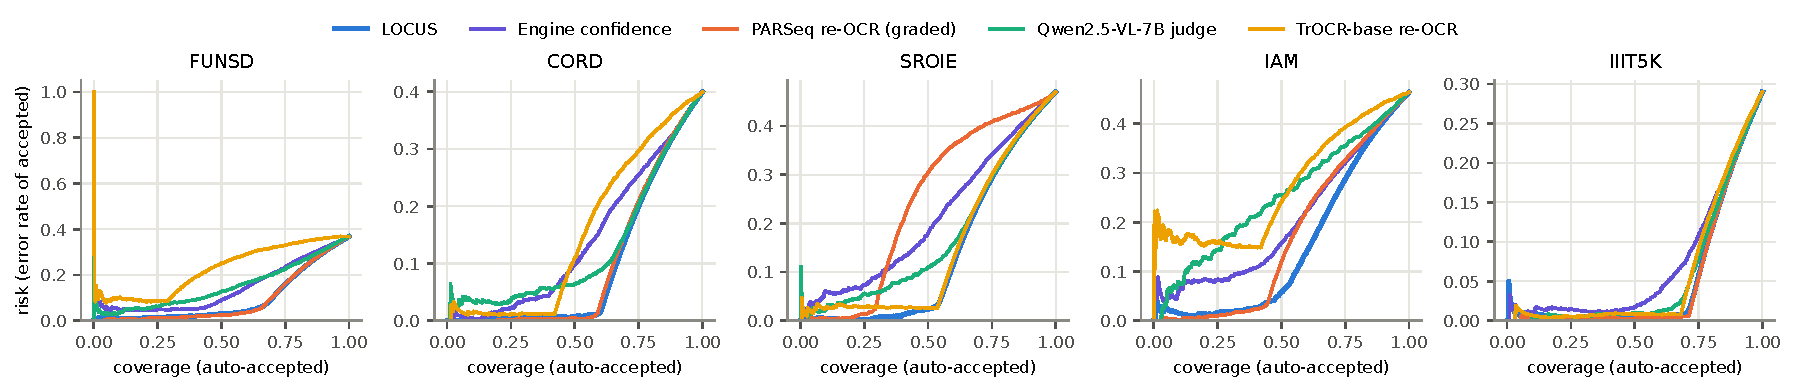
\includegraphics[width=0.78\linewidth]{figs/risk_coverage.pdf}
\caption{\textbf{Risk--coverage.} Error rate among auto-accepted words as a function of the fraction accepted ($k=25$;
lower is better).}
\label{fig:rc}
\end{figure}

\begin{table}[t]\centering
\caption{\textbf{Human-review workload}: percentage of all words that must be reviewed so that the automatically
accepted words reach the target precision ($k=25$; lower is better).}
\label{tab:review}
\scriptsize\setlength{\tabcolsep}{4pt}
\begin{minipage}[t]{0.49\linewidth}\centering
\begin{tabular}{llccc}\toprule
Dataset & Method & 90\% & 95\% & 98\%\\\midrule
\tabinput{tables/review_cost_a.tex}
\bottomrule\end{tabular}
\end{minipage}\hfill
\begin{minipage}[t]{0.49\linewidth}\centering
\begin{tabular}{llccc}\toprule
Dataset & Method & 90\% & 95\% & 98\%\\\midrule
\tabinput{tables/review_cost_b.tex}
\bottomrule\end{tabular}
\end{minipage}
\end{table}

\begin{table}[t]\centering
\caption{\textbf{Repair and cost.} Left: share of real errors whose truth lies in $G(h)$, and top-1 exact repair accuracy
(\%) of substituting TrOCR's reading, PARSeq's reading, or \ours{}' label-free proposal. Right: measured throughput on
256 FUNSD words on one RTX A6000.}
\label{tab:repair}
\footnotesize\setlength{\tabcolsep}{3pt}
\begin{minipage}[t]{0.47\linewidth}\centering
\resizebox{\linewidth}{!}{\begin{tabular}{lccccc}\toprule
Dataset & errors & in $G(h)$ & TrOCR & PARSeq & \ours{}\\\midrule
\tabinput{tables/repair.tex}
\bottomrule\end{tabular}}
\end{minipage}\hfill
\begin{minipage}[t]{0.51\linewidth}\centering
\phantomsection\label{tab:runtime}
\resizebox{\linewidth}{!}{\begin{tabular}{lcc}\toprule
Component & parameters & words/s\\\midrule
\tabinput{tables/runtime.tex}
\bottomrule\end{tabular}}
\end{minipage}
\end{table}
